% Created by tikzDevice version 0.10.1 on 2016-08-19 15:27:28
% !TEX encoding = UTF-8 Unicode
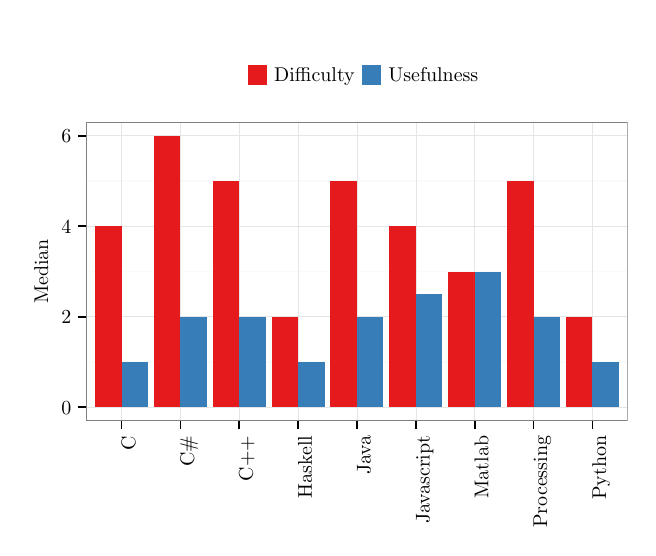
\begin{tikzpicture}[x=1pt,y=1pt]
\definecolor{fillColor}{RGB}{255,255,255}
\path[use as bounding box,fill=fillColor,fill opacity=0.00] (0,0) rectangle (216.81,180.67);
\begin{scope}
\path[clip] (  0.00,  0.00) rectangle (216.81,180.67);
\definecolor{drawColor}{RGB}{255,255,255}
\definecolor{fillColor}{RGB}{255,255,255}

\path[draw=drawColor,line width= 0.6pt,line join=round,line cap=round,fill=fillColor] ( -0.00,  0.00) rectangle (216.81,180.68);
\end{scope}
\begin{scope}
\path[clip] ( 21.16, 38.59) rectangle (216.81,146.53);
\definecolor{fillColor}{RGB}{255,255,255}

\path[fill=fillColor] ( 21.16, 38.59) rectangle (216.81,146.53);
\definecolor{drawColor}{gray}{0.98}

\path[draw=drawColor,line width= 0.6pt,line join=round] ( 21.16, 59.85) --
	(216.81, 59.85);

\path[draw=drawColor,line width= 0.6pt,line join=round] ( 21.16, 92.56) --
	(216.81, 92.56);

\path[draw=drawColor,line width= 0.6pt,line join=round] ( 21.16,125.27) --
	(216.81,125.27);
\definecolor{drawColor}{gray}{0.90}

\path[draw=drawColor,line width= 0.2pt,line join=round] ( 21.16, 43.50) --
	(216.81, 43.50);

\path[draw=drawColor,line width= 0.2pt,line join=round] ( 21.16, 76.21) --
	(216.81, 76.21);

\path[draw=drawColor,line width= 0.2pt,line join=round] ( 21.16,108.92) --
	(216.81,108.92);

\path[draw=drawColor,line width= 0.2pt,line join=round] ( 21.16,141.63) --
	(216.81,141.63);

\path[draw=drawColor,line width= 0.2pt,line join=round] ( 33.92, 38.59) --
	( 33.92,146.53);

\path[draw=drawColor,line width= 0.2pt,line join=round] ( 55.18, 38.59) --
	( 55.18,146.53);

\path[draw=drawColor,line width= 0.2pt,line join=round] ( 76.45, 38.59) --
	( 76.45,146.53);

\path[draw=drawColor,line width= 0.2pt,line join=round] ( 97.72, 38.59) --
	( 97.72,146.53);

\path[draw=drawColor,line width= 0.2pt,line join=round] (118.98, 38.59) --
	(118.98,146.53);

\path[draw=drawColor,line width= 0.2pt,line join=round] (140.25, 38.59) --
	(140.25,146.53);

\path[draw=drawColor,line width= 0.2pt,line join=round] (161.52, 38.59) --
	(161.52,146.53);

\path[draw=drawColor,line width= 0.2pt,line join=round] (182.78, 38.59) --
	(182.78,146.53);

\path[draw=drawColor,line width= 0.2pt,line join=round] (204.05, 38.59) --
	(204.05,146.53);
\definecolor{fillColor}{RGB}{55,126,184}

\path[fill=fillColor] ( 33.92, 43.50) rectangle ( 43.49, 59.85);
\definecolor{fillColor}{RGB}{228,26,28}

\path[fill=fillColor] ( 24.35, 43.50) rectangle ( 33.92,108.92);
\definecolor{fillColor}{RGB}{55,126,184}

\path[fill=fillColor] ( 55.18, 43.50) rectangle ( 64.75, 76.21);
\definecolor{fillColor}{RGB}{228,26,28}

\path[fill=fillColor] ( 45.61, 43.50) rectangle ( 55.18,141.63);
\definecolor{fillColor}{RGB}{55,126,184}

\path[fill=fillColor] ( 76.45, 43.50) rectangle ( 86.02, 76.21);
\definecolor{fillColor}{RGB}{228,26,28}

\path[fill=fillColor] ( 66.88, 43.50) rectangle ( 76.45,125.27);
\definecolor{fillColor}{RGB}{55,126,184}

\path[fill=fillColor] ( 97.72, 43.50) rectangle (107.29, 59.85);
\definecolor{fillColor}{RGB}{228,26,28}

\path[fill=fillColor] ( 88.15, 43.50) rectangle ( 97.72, 76.21);
\definecolor{fillColor}{RGB}{55,126,184}

\path[fill=fillColor] (118.98, 43.50) rectangle (128.55, 76.21);
\definecolor{fillColor}{RGB}{228,26,28}

\path[fill=fillColor] (109.41, 43.50) rectangle (118.98,125.27);
\definecolor{fillColor}{RGB}{55,126,184}

\path[fill=fillColor] (140.25, 43.50) rectangle (149.82, 84.38);
\definecolor{fillColor}{RGB}{228,26,28}

\path[fill=fillColor] (130.68, 43.50) rectangle (140.25,108.92);
\definecolor{fillColor}{RGB}{55,126,184}

\path[fill=fillColor] (161.52, 43.50) rectangle (171.09, 92.56);
\definecolor{fillColor}{RGB}{228,26,28}

\path[fill=fillColor] (151.95, 43.50) rectangle (161.52, 92.56);
\definecolor{fillColor}{RGB}{55,126,184}

\path[fill=fillColor] (182.78, 43.50) rectangle (192.35, 76.21);
\definecolor{fillColor}{RGB}{228,26,28}

\path[fill=fillColor] (173.21, 43.50) rectangle (182.78,125.27);
\definecolor{fillColor}{RGB}{55,126,184}

\path[fill=fillColor] (204.05, 43.50) rectangle (213.62, 59.85);
\definecolor{fillColor}{RGB}{228,26,28}

\path[fill=fillColor] (194.48, 43.50) rectangle (204.05, 76.21);
\definecolor{drawColor}{gray}{0.50}

\path[draw=drawColor,line width= 0.6pt,line join=round,line cap=round] ( 21.16, 38.59) rectangle (216.81,146.53);
\end{scope}
\begin{scope}
\path[clip] (  0.00,  0.00) rectangle (216.81,180.67);
\definecolor{drawColor}{RGB}{0,0,0}

\node[text=drawColor,anchor=base east,inner sep=0pt, outer sep=0pt, scale=  0.72] at ( 15.76, 41.02) {0};

\node[text=drawColor,anchor=base east,inner sep=0pt, outer sep=0pt, scale=  0.72] at ( 15.76, 73.73) {2};

\node[text=drawColor,anchor=base east,inner sep=0pt, outer sep=0pt, scale=  0.72] at ( 15.76,106.44) {4};

\node[text=drawColor,anchor=base east,inner sep=0pt, outer sep=0pt, scale=  0.72] at ( 15.76,139.15) {6};
\end{scope}
\begin{scope}
\path[clip] (  0.00,  0.00) rectangle (216.81,180.67);
\definecolor{drawColor}{RGB}{0,0,0}

\path[draw=drawColor,line width= 0.6pt,line join=round] ( 18.16, 43.50) --
	( 21.16, 43.50);

\path[draw=drawColor,line width= 0.6pt,line join=round] ( 18.16, 76.21) --
	( 21.16, 76.21);

\path[draw=drawColor,line width= 0.6pt,line join=round] ( 18.16,108.92) --
	( 21.16,108.92);

\path[draw=drawColor,line width= 0.6pt,line join=round] ( 18.16,141.63) --
	( 21.16,141.63);
\end{scope}
\begin{scope}
\path[clip] (  0.00,  0.00) rectangle (216.81,180.67);
\definecolor{drawColor}{RGB}{0,0,0}

\path[draw=drawColor,line width= 0.6pt,line join=round] ( 33.92, 35.59) --
	( 33.92, 38.59);

\path[draw=drawColor,line width= 0.6pt,line join=round] ( 55.18, 35.59) --
	( 55.18, 38.59);

\path[draw=drawColor,line width= 0.6pt,line join=round] ( 76.45, 35.59) --
	( 76.45, 38.59);

\path[draw=drawColor,line width= 0.6pt,line join=round] ( 97.72, 35.59) --
	( 97.72, 38.59);

\path[draw=drawColor,line width= 0.6pt,line join=round] (118.98, 35.59) --
	(118.98, 38.59);

\path[draw=drawColor,line width= 0.6pt,line join=round] (140.25, 35.59) --
	(140.25, 38.59);

\path[draw=drawColor,line width= 0.6pt,line join=round] (161.52, 35.59) --
	(161.52, 38.59);

\path[draw=drawColor,line width= 0.6pt,line join=round] (182.78, 35.59) --
	(182.78, 38.59);

\path[draw=drawColor,line width= 0.6pt,line join=round] (204.05, 35.59) --
	(204.05, 38.59);
\end{scope}
\begin{scope}
\path[clip] (  0.00,  0.00) rectangle (216.81,180.67);
\definecolor{drawColor}{RGB}{0,0,0}

\node[text=drawColor,rotate= 90.00,anchor=base east,inner sep=0pt, outer sep=0pt, scale=  0.72] at ( 38.88, 33.19) {C};

\node[text=drawColor,rotate= 90.00,anchor=base east,inner sep=0pt, outer sep=0pt, scale=  0.72] at ( 60.14, 33.19) {C\#};

\node[text=drawColor,rotate= 90.00,anchor=base east,inner sep=0pt, outer sep=0pt, scale=  0.72] at ( 81.41, 33.19) {C++};

\node[text=drawColor,rotate= 90.00,anchor=base east,inner sep=0pt, outer sep=0pt, scale=  0.72] at (102.68, 33.19) {Haskell};

\node[text=drawColor,rotate= 90.00,anchor=base east,inner sep=0pt, outer sep=0pt, scale=  0.72] at (123.94, 33.19) {Java};

\node[text=drawColor,rotate= 90.00,anchor=base east,inner sep=0pt, outer sep=0pt, scale=  0.72] at (145.21, 33.19) {Javascript};

\node[text=drawColor,rotate= 90.00,anchor=base east,inner sep=0pt, outer sep=0pt, scale=  0.72] at (166.48, 33.19) {Matlab};

\node[text=drawColor,rotate= 90.00,anchor=base east,inner sep=0pt, outer sep=0pt, scale=  0.72] at (187.74, 33.19) {Processing};

\node[text=drawColor,rotate= 90.00,anchor=base east,inner sep=0pt, outer sep=0pt, scale=  0.72] at (209.01, 33.19) {Python};
\end{scope}
\begin{scope}
\path[clip] (  0.00,  0.00) rectangle (216.81,180.67);
\definecolor{drawColor}{RGB}{0,0,0}

\node[text=drawColor,rotate= 90.00,anchor=base,inner sep=0pt, outer sep=0pt, scale=  0.72] at (  7.36, 92.56) {Median};
\end{scope}
\begin{scope}
\path[clip] (  0.00,  0.00) rectangle (216.81,180.67);
\definecolor{fillColor}{RGB}{255,255,255}

\path[fill=fillColor] ( 70.86,155.07) rectangle (167.11,172.14);
\end{scope}
\begin{scope}
\path[clip] (  0.00,  0.00) rectangle (216.81,180.67);
\definecolor{fillColor}{RGB}{228,26,28}

\path[fill=fillColor] ( 79.45,160.05) rectangle ( 86.57,167.16);
\end{scope}
\begin{scope}
\path[clip] (  0.00,  0.00) rectangle (216.81,180.67);
\definecolor{fillColor}{RGB}{55,126,184}

\path[fill=fillColor] (120.70,160.05) rectangle (127.81,167.16);
\end{scope}
\begin{scope}
\path[clip] (  0.00,  0.00) rectangle (216.81,180.67);
\definecolor{drawColor}{RGB}{0,0,0}

\node[text=drawColor,anchor=base west,inner sep=0pt, outer sep=0pt, scale=  0.72] at ( 89.08,161.12) {Difficulty};
\end{scope}
\begin{scope}
\path[clip] (  0.00,  0.00) rectangle (216.81,180.67);
\definecolor{drawColor}{RGB}{0,0,0}

\node[text=drawColor,anchor=base west,inner sep=0pt, outer sep=0pt, scale=  0.72] at (130.33,161.12) {Usefulness};
\end{scope}
\end{tikzpicture}
